\begin{saveblock}{ninglinspoFragment1}
    \begin{Verbatim}[tabsize=4,gobble=4]
    {{Infobox rivier
            | naam          = Ninglinspo
            | afbeelding    = Ninglinspo - arrivée d
            | onderschrift  = De Ninglinspo niet ver
            | lengte        = 15
            | hoogte        = 420
            | hoogtemonding = 270
            | verhang       = 
            | debiet        = 
    \end{Verbatim}
\end{saveblock}

\begin{saveblock}{ninglinspoFragment2}
    \begin{Verbatim}[tabsize=4,gobble=8]
    De oorspronkelijke naam is eigenlijk de "Doulneu
    een Els. Er werd reeds gesproken over de rivier
    charter van [[Sigibert III]].
    <ref>informatiebord aan de monding van de Ningli
    \end{Verbatim}
\end{saveblock}

\begin{frame}
    \frametitle{Code vs \lang,Visual,Visueel,}

    % \begin{columns}
    %    \begin{column}{0.45\textwidth}
    %\centering
    \adjustbox{
        trim=0pt 0pt 5em 0pt,
        max height=0.9\textheight,max width=0.5\linewidth,
        %fbox=1pt 0pt 2pt,
        cframe=green!50!white 0.5pt 0pt 2pt,
        valign=M
    }{
        \useblock{ninglinspoFragment1}
    }%
    %\hspace{2pt}%
    \adjustbox{
        cframe=blue!50!white 0.5pt 0pt 0pt,
        valign=M
    }{%
        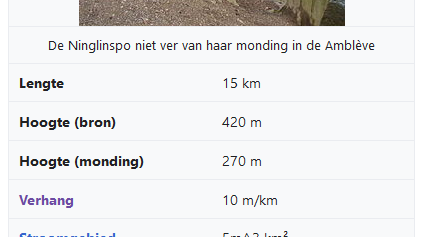
\includegraphics[
            trim=7pt 0pt 7pt 0pt,clip,
            height=0.5\textheight,width=0.5\linewidth,keepaspectratio]{assets/wikipediaInfobox.png}%
    }
    \vspace{5pt}

    \adjustbox{
        trim=0pt 0pt 5em 0pt,
        max height=0.9\textheight, max width=0.5\linewidth,
        %fbox=1pt 0pt 2pt,
        cframe=green!50!white 0.5pt 0pt 2pt,
        valign=M
    }{
        \useblock{ninglinspoFragment2}
    }%
    \adjustbox{
        cframe=blue!50!white 0.5pt 0pt 0pt,
        valign=M
    }{%
        
\includegraphics[height=0.5\textheight,width=0.5\linewidth,keepaspectratio]{assets/wikipediaHyperAndFootnotes.png}%
    }
\end{frame}
